% A rudimentary beamer template for C2SM presentations - HvW-09-07-2013
\documentclass[xcolor=pdftex,dvipsnames,table]{beamer}
\usepackage[utf8]{inputenc}
\usepackage[T1]{fontenc}
\usepackage{graphicx}
\usepackage{fancybox}
\usepackage{booktabs}
\usepackage{xcolor,colortbl}

%% Setting up a very basic template %%%%%%%%%%%%%%%%%%%%%%%%%%%%%%%%%%%%%%%%%%%%
%% Maybe ignore this part for now   %%%%%%%%%%%%%%%%%%%%%%%%%%%%%%%%%%%%%%%%%%%%

%% The theme is pace optimizing: no navigation symbols, no footline, no
%% header. Frametitles have offcial eth-color #8, which appears to
%% match (says the aethetically handicapped), both the pale C2SM-blue
%% and the black block title background.
\setbeamersize{text margin left=1em,text margin right=1em}
\definecolor{eth8}{RGB}{0,122,150}
\usecolortheme[RGB={63,63,63}]{structure}
\setbeamertemplate{navigation symbols}{}
\setbeamertemplate{footline}{}
\setbeamercolor{frametitle}{bg=eth8,fg=white}
\setbeamerfont{frametitle}{series=\bfseries}
\useinnertheme[shadow]{rounded}
\setbeamercolor{block title}{use=structure,fg=white,bg=structure.fg!75!black}
\setbeamercolor{block title alerted}{use=alerted text,fg=white,bg=alerted text.fg!75!black}
\setbeamercolor{block title example}{use=example text,fg=white,bg=example text.fg!75!black}
\setbeamercolor{block body}{parent=normal text,use=block title,bg=block title.bg!5!bg}
\setbeamercolor{block body alerted}{parent=normal text,use=block title alerted,
  bg=block title alerted.bg!15!bg}
\setbeamercolor{block body example}{parent=normal text,use=block title example,
  bg=block title example.bg!5!bg}

%% chop of something from the frametitle to make space for C2SM logo 
\setbeamertemplate{frametitle} {
  \begin{beamercolorbox}[wd=0.86\textwidth,leftskip=.3cm,rounded=true]{frametitle}
    \insertframetitle
  \end{beamercolorbox}
}

%% this is some trickery to be able to change the margins temporally.
%% used to put the C2SM motive onto the title page
\newenvironment{changemargin}[2]{%
  \begin{list}{}{%
    \setlength{\topsep}{0pt}%
    \setlength{\leftmargin}{#1}%
    \setlength{\rightmargin}{#2}%
    \setlength{\listparindent}{\parindent}%
    \setlength{\itemindent}{\parindent}%
    \setlength{\parsep}{\parskip}%
  }%
\item[]}{\end{list}}

%% the title page
\defbeamertemplate*{title page}{customized}[1][] {
%%%% the two logos on top of the title page
  \raisebox{-0.3cm}{\parbox{1.018\textwidth} {
      \hspace{-0.5em}
      
\includegraphics[height=1.1cm]{pics_template/c2sm_3.png}
      \hfill
      \raisebox{0.6cm}{
\includegraphics[height=0.35cm]{pics_template/eth_logo_kurz_pos.pdf}}
    }
  }

%%%% the title
  \begin{center}
    \vspace{-0.76in} % move the title up and down as needed
                    % If the title takes up too much vertical space, then
                    % the C2SM - motive wilkl be pushed down and the reference
                    % to the picture source (NASA) disappears!
      \begin{minipage}[t][0.5\textheight][c]{0.71\textwidth}
        \begin{center}
          \usebeamerfont{title}{\textcolor{eth8}\inserttitle\par}
          \usebeamerfont{subtitle}\usebeamercolor[fg]{subtitle}\insertsubtitle\par
          \bigskip
          \usebeamerfont{author}\insertauthor\par
          \usebeamerfont{institute}\insertinstitute\par
          \bigskip
          \usebeamerfont{date}\insertdate\par
        \end{center}
      \end{minipage}
  \end{center}

%%%% The C2SM - motive
  \begin{changemargin}{-1em}{-1em}
    {\centering 
      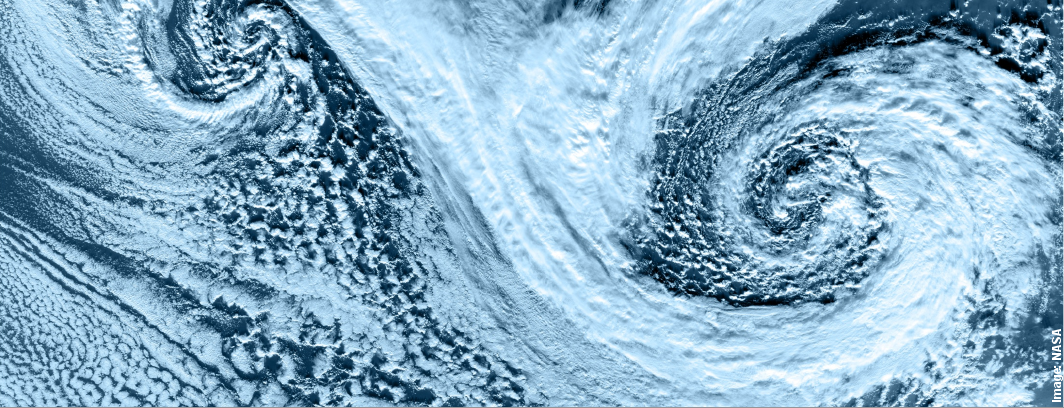
\includegraphics[width=\paperwidth,height=0.54
      \textheight]{pics_template/c2sm_background.png}\\
    }
  \end{changemargin}
}

% %%%%%%%%%%%%%%%%%%%%%%%%%%%%%%%  here starts your content %%%%%%%%%%%%%%%%%%%%
% %%%%%%%%%%%%%%%%%%%%%%%%%%%%%%%%%%%%%%%%%%%%%%%%%%%%%%%%%%%%%%%%%%%%%%%%%%%%%%
\title{C2SM workshop\\Scientific Programming in Python}
\author{
  Harald von Waldow {\tiny(C2SM/ETHZ)}\\
  Nicolas Piaget {\tiny(Atm.Dyn./ETHZ)}\\
  Timm Gross {\tiny(GIUB/UNIBE)}
}



\date{2015--02--11}

\begin{document}

\setbeamercovered{dynamic}

\begin{frame}
  \titlepage%
\end{frame}

%% This puts the C2SM - logo in the top right corner
%% Can someone put that into a new command?
  \usebackgroundtemplate{
    \raisebox{-0.7cm}{
      \parbox{\paperwidth}{\raggedleft
\includegraphics[height=1.1cm]{pics_template/c2sm_3.png}\ \ }
    }
  }

\usebackgroundtemplate{}
\begin{frame}
  \frametitle{Schedule}

\small{
\begin{tabular}{p{1cm}|l|p{2cm}}

  \rowcolor{lightgray}09:30 & Welcome, organizational matters & Harald\\
  %\midrule
  \rowcolor{lightgray}09:45 & Python --- The big picture & Harald\\
  %\midrule
  %% \rowcolor{lightgray}10:00 & \parbox[t]{6cm}{Python development tools\\The IPython Notebook --- First steps} & \parbox[t]{1cm}{Harald\\Bas}\\

  \rowcolor{lightgray}10:00 & Python development tools & Harald\\
  % \midrule
  \rowcolor{cyan}10:15 & \textbf{Exercise 1}: The IPython Notebook & Harald/Nicolas\\
  %\midrule
  \rowcolor{orange}10:45 & Coffee Break \textbf{15 min}&\\
  %\midrule
  \rowcolor{cyan}11:00 & \textbf{Exercise 2}: Basic Python & Harald\\
  %\midrule
  \rowcolor{orange}12:00 & Lunch Break \textbf{1 h} &\\
  %\midrule
  \rowcolor{cyan}13:00 & \textbf{Exercise 3}: Numpy, Scipy, Matplotlib, netCDF4 & Nicolas\\
  %\midrule
  \rowcolor{orange}14:30 & Coffee Break \textbf{15 min}&\\
  %\midrule
  \rowcolor{cyan}14:45 & \textbf{Exercise 4}: More fun with trajectory plots & Nicolas\\
  %\midrule
  \rowcolor{orange}15:45 & Coffee Break \textbf{15 min}&\\
  %\midrule
  \rowcolor{cyan}16:00 & \textbf{Exercise 5}: Easy mapping \& projecting & Harald\\
  %\midrule
  \rowcolor{lightgray}17:00 & Other packages, Outlook & Harald\\
  \rowcolor{lightgray}17:15 & Wrap up, Discussion, Questions, Feedback & Harald\\
  %\midrule
  \rowcolor{lightgray}17:30? & End &\\

\end{tabular}
}
\end{frame}

\begin{frame}
  \frametitle{Organizational Matters}

%\visible<2->{
  \begin{block}{IT-setup}
    \only<1>{
      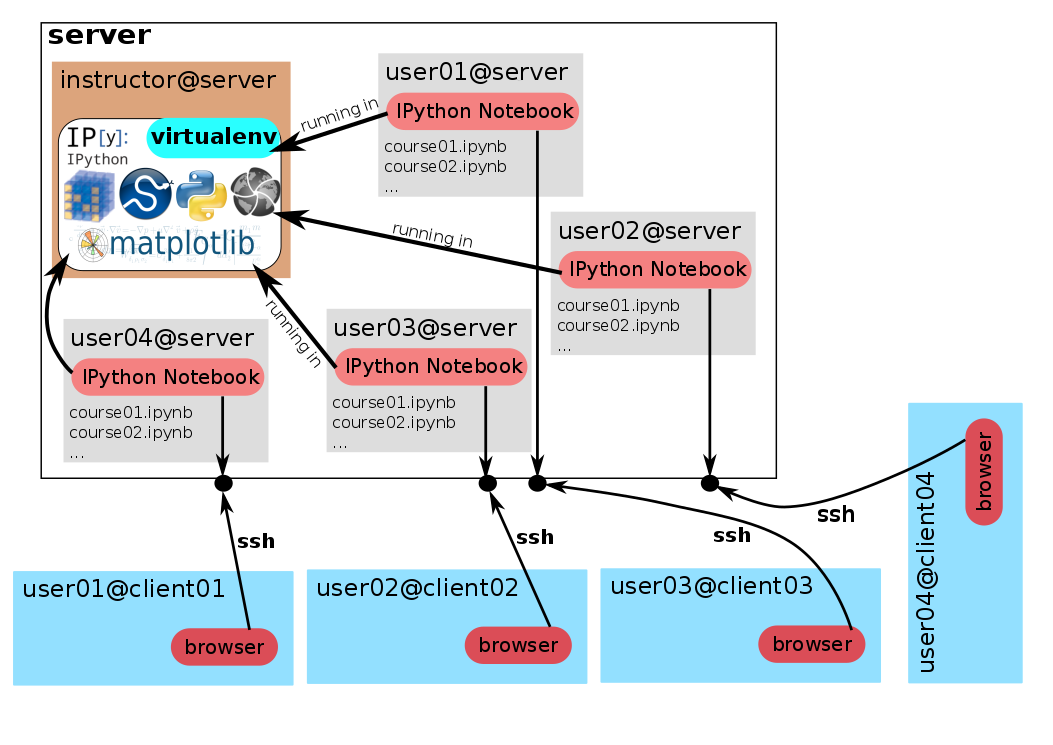
\includegraphics[width=0.98\textwidth]{setup.png}
    }
    \only<2> {
      \footnotesize
      \begin{itemize}
      \item On your local desktop runs a browser.
      \item The browser connects to a local port (7777), which is forwarded to a port on our server.
      \item On that server runs the IPython-process, one for everybody, and all data resides there.
      \item That server is \texttt{climcal04.unibe.ch}. You should not need to worry about that.
      \end{itemize}
    }
  \end{block}
%}

\end{frame}

\begin{frame}
  \frametitle{Organizational Matters}
  \begin{block}{Login}
    \begin{itemize}
      \item username: \texttt{pywsXX}
      \item \texttt{XX} is \texttt{01} \ldots \texttt{17}  
      \item password: \texttt{--- censored ---}
      \item After login start a terminal window
      \item type ``./startup''
      \item the browser should start and load the proper page.
    \end{itemize}
  \end{block}
\end{frame}

\begin{frame}
  \frametitle{Python --- the big picture}
  \begin{block}{History, Versions}
    \begin{itemize}
      \item A young and fast moving language by Guido van Rossum:\\
        \begin{itemize}
          \item Python 1.0: 1994
          \item Python 2.0: 2000
          \item<+-|alert@2> Python 2.7: 2010
          \item Python 3.0: 2008
          \item Python 3.4: 2014
        \end{itemize}
      \item<2-> Python 3.x is incompatible with 2.x.
      \item<2-> New, large projects should be written in 3.x.
      \item<2-> For research code, often depending on exotic modules, use 2.7.
      \item<2-> Some new features can be made available in 2.7 using\\ \texttt{from \_\_future\_\_ import XY}
    \end{itemize}
  \end{block}
\end{frame}

\begin{frame}
  \frametitle{Python --- the big picture}
  \begin{block}{Classification}
    \begin{itemize}[<+->]
    \item interpreted
    \item general-purpose, high-level
    \item dynamically typed
    \item garbage-collection
    \item multi-paradigm:
      \begin{itemize}[<+->]
          \item object-orented
          \item functional programming features
        \end{itemize}
    \end{itemize}
  \end{block}
\visible<8->{
  \begin{block}{Features}
  \begin{itemize}[<+->]
  \item \textbf{optimal for fast development} 
  \item documentation well integrated with code
  \item clean, simple, intuitive
  \item expressive (= less lines of code)
  \item scales well with project size
  \end{itemize}
  \end{block}}
\end{frame}

\begin{frame}
  \frametitle{Python --- the big picture}
  \begin{block}{Advantages for scientific computing}
  \begin{itemize}[<+->]
  \item large and fast growing user community
  \item large and fast growing number of libraries for sci. com.
  \item well integrated with ``bread-and-butter'' codes, such as\\
    BLAS, LAPACK, Netlib standards such as ODEPACK, \ldots
  \item highly extensible, large collection of add-on packages
  \item easy communication with R, C, Fortran, \ldots
  \end{itemize}
  \end{block}
\end{frame}

\begin{frame}
  \frametitle{Python --- the big picture}
  \begin{block}{When to use Python?}
    \textbf{ALWAYS!}\\
    except:
    \begin{itemize}[<+->]
    \item You need the speed of C or Fortran
    \item You can re-use significant code written in other languages.
    \item You do HPC (using MPI, OpenMP)
    \item Your can profit from a non-Python tradition in your field or workgroup.
    \item Something else is better for the task, \ldots
    \end{itemize}
  \end{block}
\visible<6->{
  \begin{block}{Other interpreted languages to consider}
    \begin{itemize}[<+->]
    \item R: lingua franca of statistics. There is no choice for advanced stats.
    \item You better know Python \textbf{and} R.
    \item Matlab: Some specialized toolboxes have (yet) no counterpart in Python.
    \end{itemize}
  \end{block}}
\end{frame}

\begin{frame}
  \frametitle{Python --- the big picture}
  \begin{block}{Philosophy}
    The Zen of Python (try \texttt{``import this''})
    \begin{itemize}[<+->]
    \item Beautiful is better than ugly.
    \item Simple is better than complex.
    \item Complex is better than complicated.
    \item Readability counts.
    \item There should be one-- and preferably only one --obvious way to do it.
    \item \ldots
    \end{itemize}
    \onslide+<7->\textbf{Python programmers strive to write \textit{pythonic}}
    \begin{itemize}[<8->]
    \item Don't get lost in beauty
    \item But if you have trouble understanding your own code \ldots
    \item \ldots after your holidays \ldots
    \item \texttt{``import this''} and re-factor a bit.
    \end{itemize}
  \end{block}
\end{frame}


\begin{frame}
  \frametitle{Basic Python}
  \begin{block}{Python shell}
    \begin{overprint}
    \onslide<1>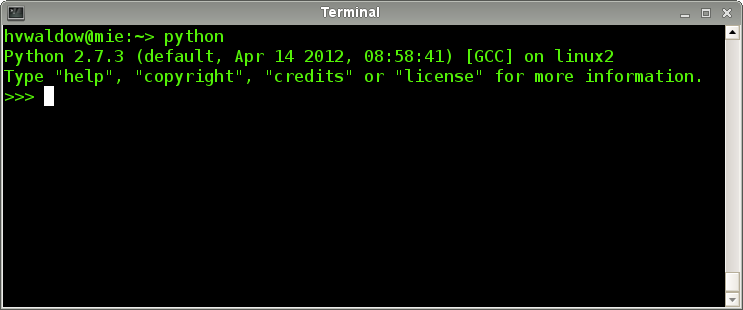
\includegraphics[width=\textwidth]{python1.png}
    \onslide<2>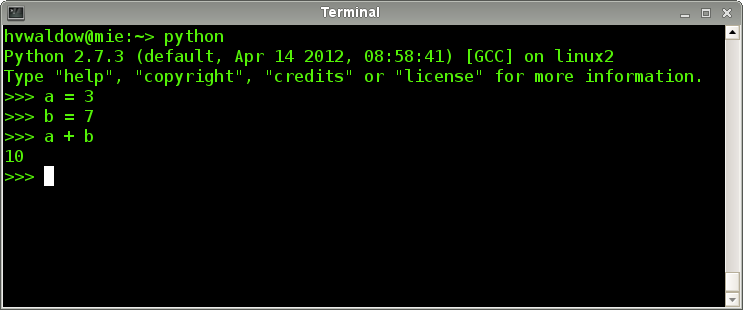
\includegraphics[width=\textwidth]{python2.png}
    \onslide<3>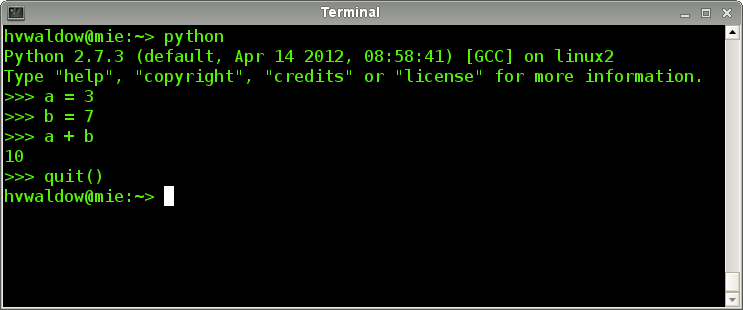
\includegraphics[width=\textwidth]{python3.png}
    \end{overprint}
    \begin{overprint}
      \onslide<1> Typing ``python'' will call the ``raw'' Python shell.
      \onslide<2> Can be used like a calculator.
      \onslide<3> Call function ``quit()'' to exit.
    \end{overprint}   
  \end{block}
\end{frame}

\begin{frame}
  \frametitle{Basic Python}
  \begin{block}{\textbf{I}Python shell}
    \begin{overprint}
    \onslide<1>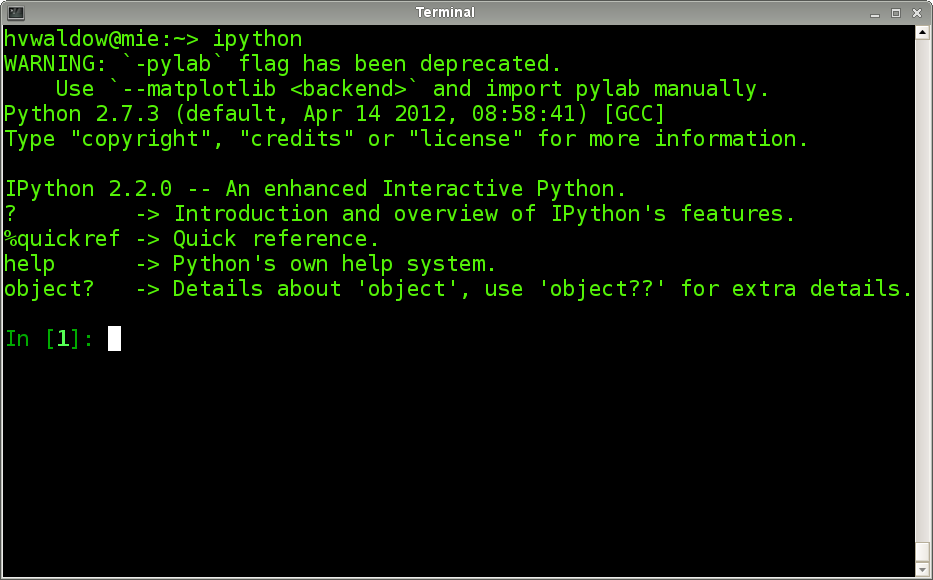
\includegraphics[width=\textwidth, height=0.75\textheight]{ipython1.png}
    \onslide<2>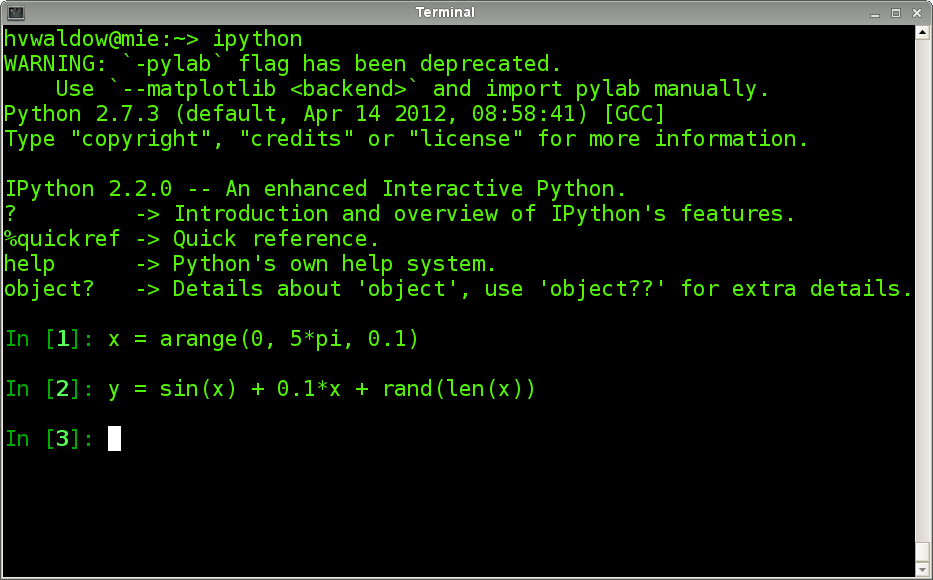
\includegraphics[width=\textwidth, height=0.75\textheight]{ipython2.png}
    \onslide<3>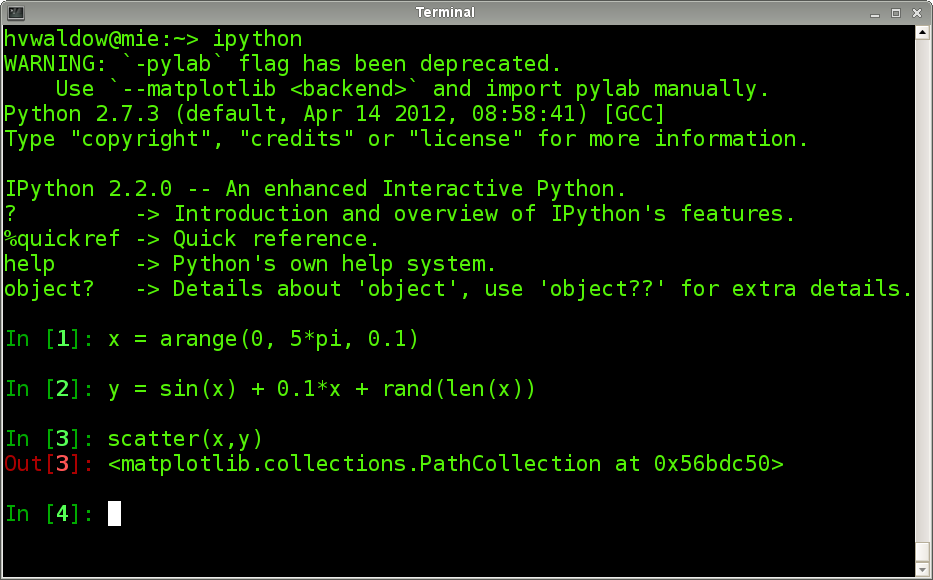
\includegraphics[width=\textwidth, height=0.75\textheight]{ipython3.png}
    \onslide<4>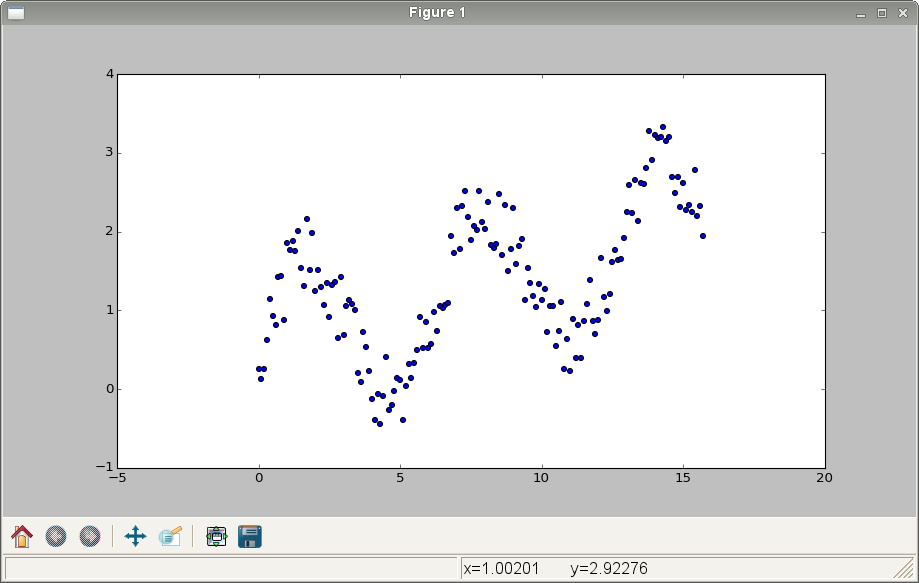
\includegraphics[width=\textwidth, height=0.75\textheight]{ipython4.png}
    \onslide<5>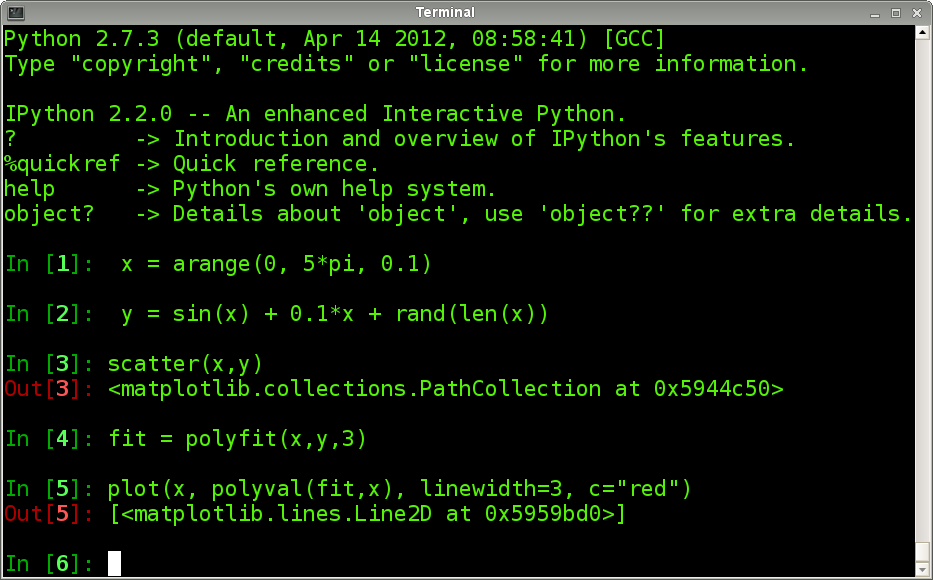
\includegraphics[width=\textwidth, height=0.75\textheight]{ipython5.png}
    \onslide<6>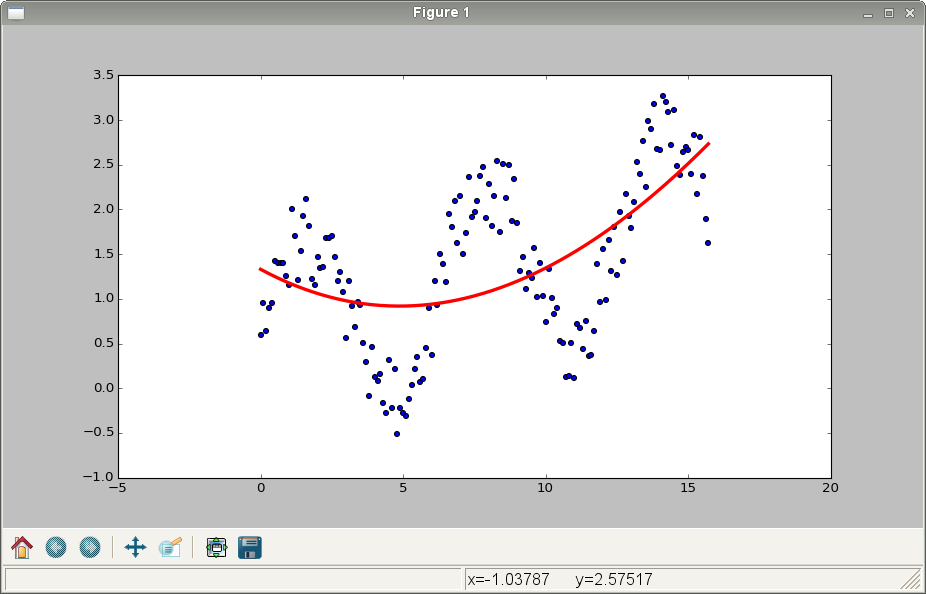
\includegraphics[width=\textwidth, height=0.75\textheight]{ipython6.png}
    \onslide<7>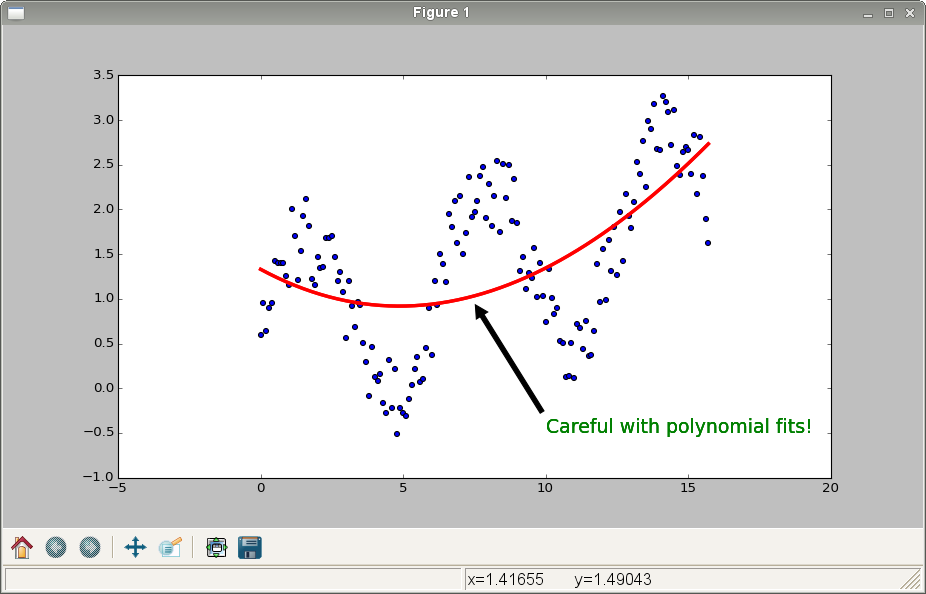
\includegraphics[width=\textwidth, height=0.75\textheight]{ipython7.png}
    \end{overprint}
    \begin{overprint}
      \onslide<1> Typing ``\textbf{i}python'' will call the IPython shell.
      \onslide<2> Math functions ``magically'' loaded.
      \onslide<3> Plot functions as well.
      \onslide<6,7> New content can be added interactively.
    \end{overprint}   
  \end{block}
\end{frame}

\begin{frame}
  \frametitle{Basic Python}
  \begin{block}{Run a python script}
    \begin{overprint}
    \onslide<1>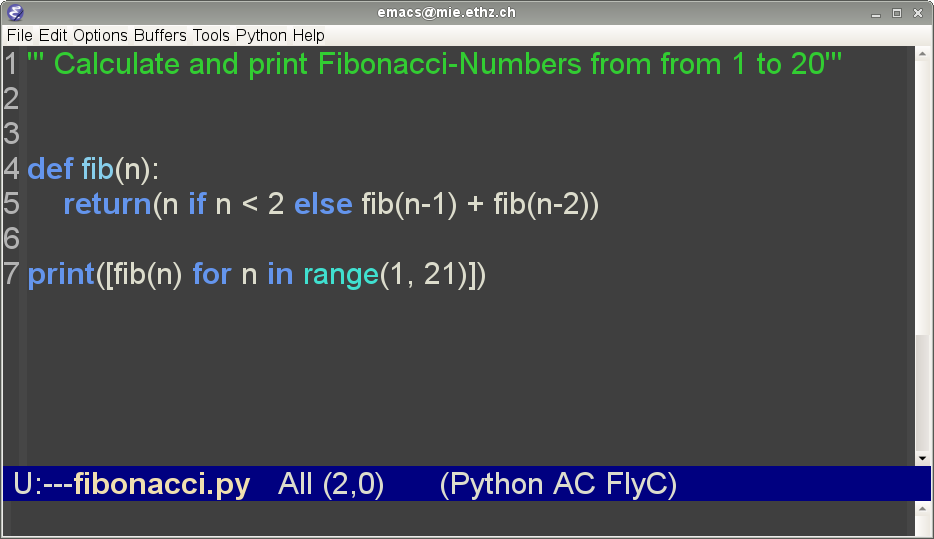
\includegraphics[width=\textwidth]{runpy1.png}
    \onslide<2>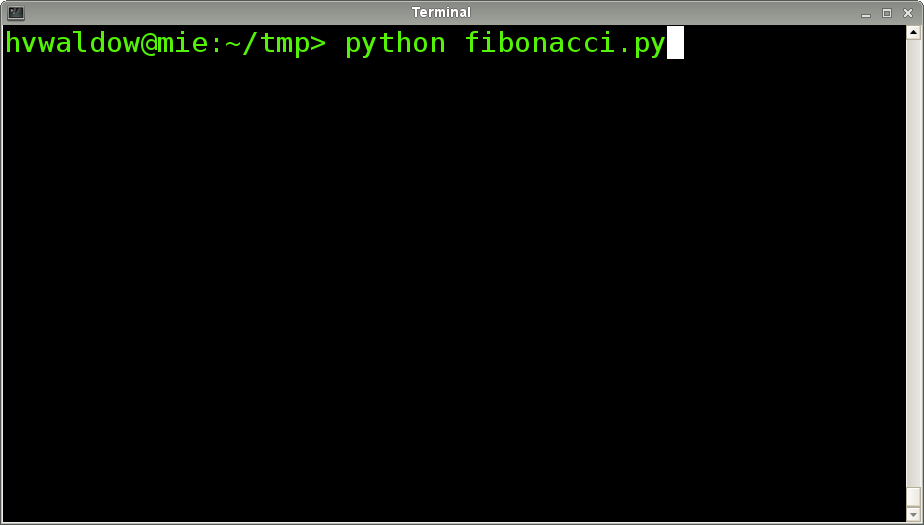
\includegraphics[width=\textwidth]{runpy2.png}
    \onslide<3>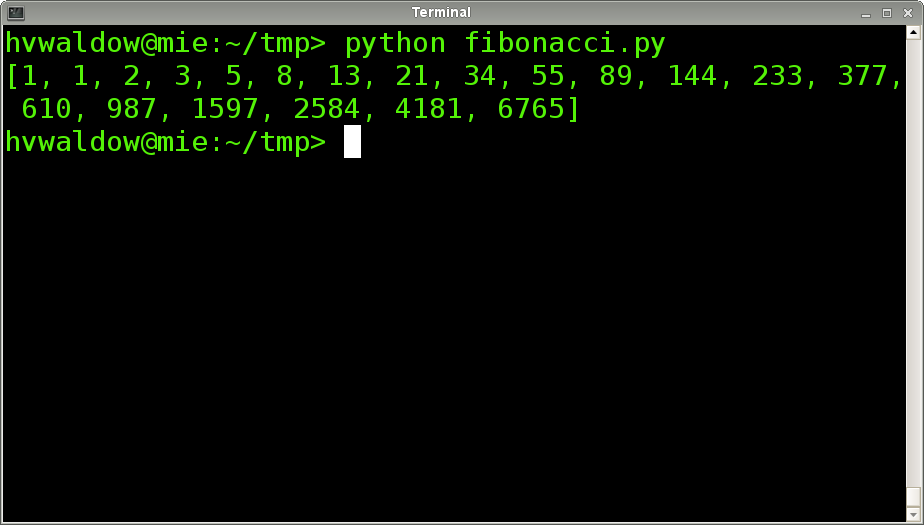
\includegraphics[width=\textwidth]{runpy3.png}
    \onslide<4>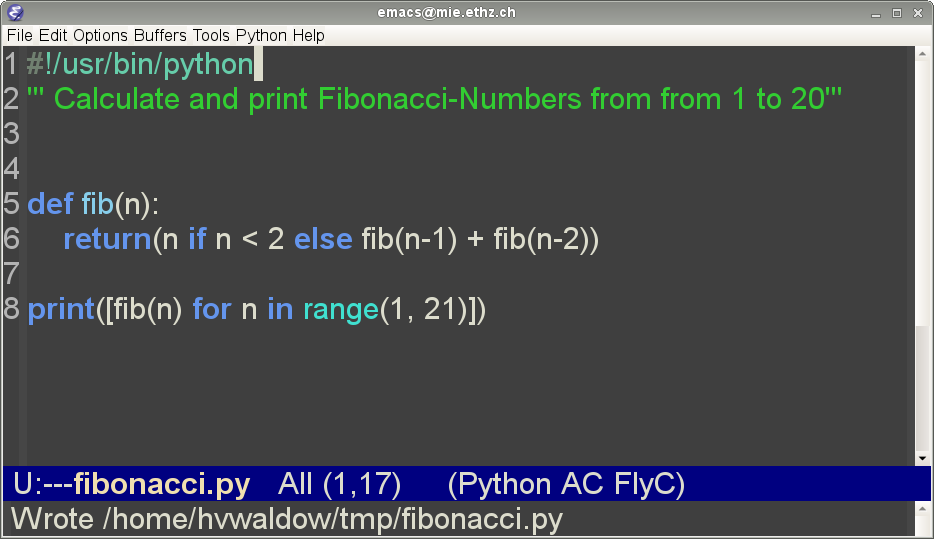
\includegraphics[width=\textwidth]{runpy4.png}
    \onslide<5>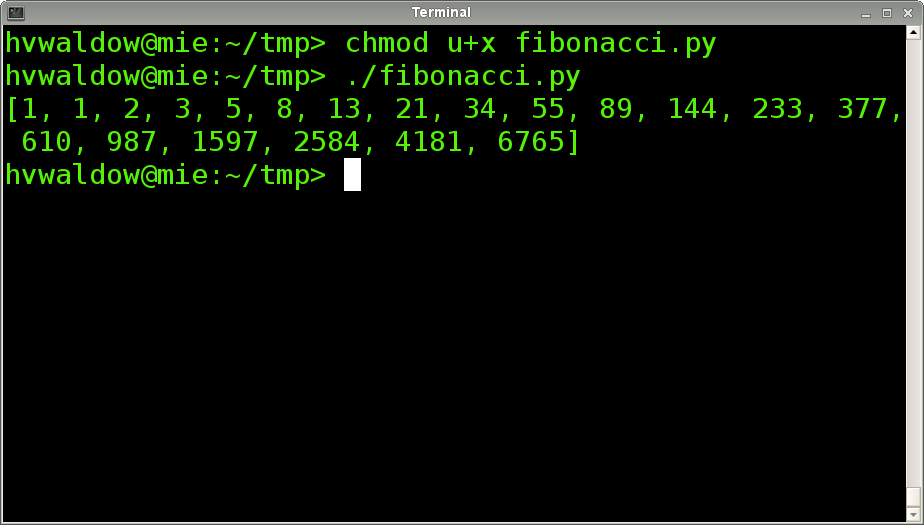
\includegraphics[width=\textwidth]{runpy5.png}
    \end{overprint}
    \begin{overprint}
      \onslide<1> Save file with ending ``.py''
      \onslide<2> Call python intepreter with filename as argument.
      \onslide<3> Output goes to stdout.
      \onslide<4> ``Shebang'' syntax works.
      \onslide<5> Make script executable and call it directly.
    \end{overprint}
  \end{block}
\end{frame}

\begin{frame}
  \frametitle{Python development tools}
  \begin{block}{Python IDEs}
        \begin{itemize}[<+->]
          \item A number of sophisticated IDEs available
          \item Like Matlab, RStudio, Visual Studio, Eclipse \ldots
          \item Can be confusing at first
          \item Many features for program development
          \item Variable inspection, debugging, \ldots
          \item Komodo IDE (commercial)
          \item Wing IDE  (commercial)
          \item Eclipse/PyDev (free)
          \item Eric (free)
          \item <+| alert@10>Spyder (free)
        \end{itemize}
  \end{block}
\end{frame}

\begin{frame}
  \frametitle{Python development tools}
  \begin{block}{Python IDEs}
    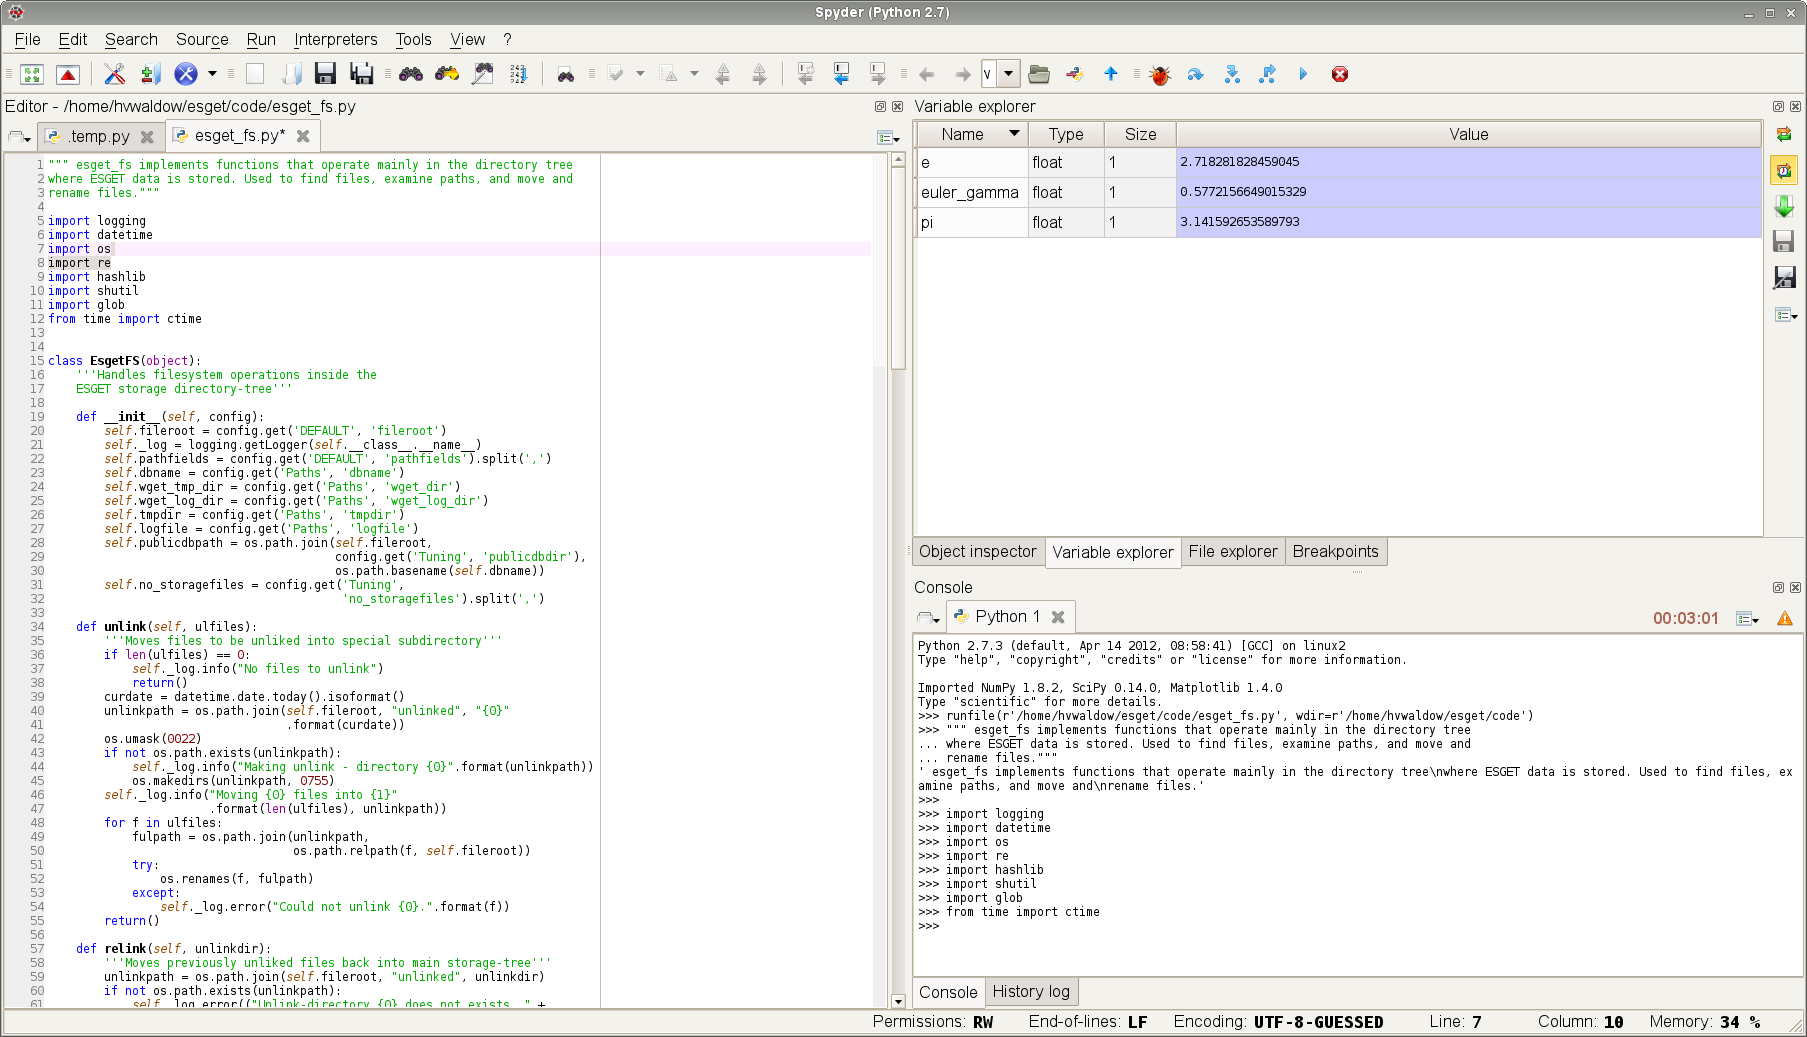
\includegraphics[width=\textwidth]{spyder.png}
  \end{block}
\end{frame}

\begin{frame}
  \frametitle{Python development tools}
  \begin{block}{Editors with plugins}
    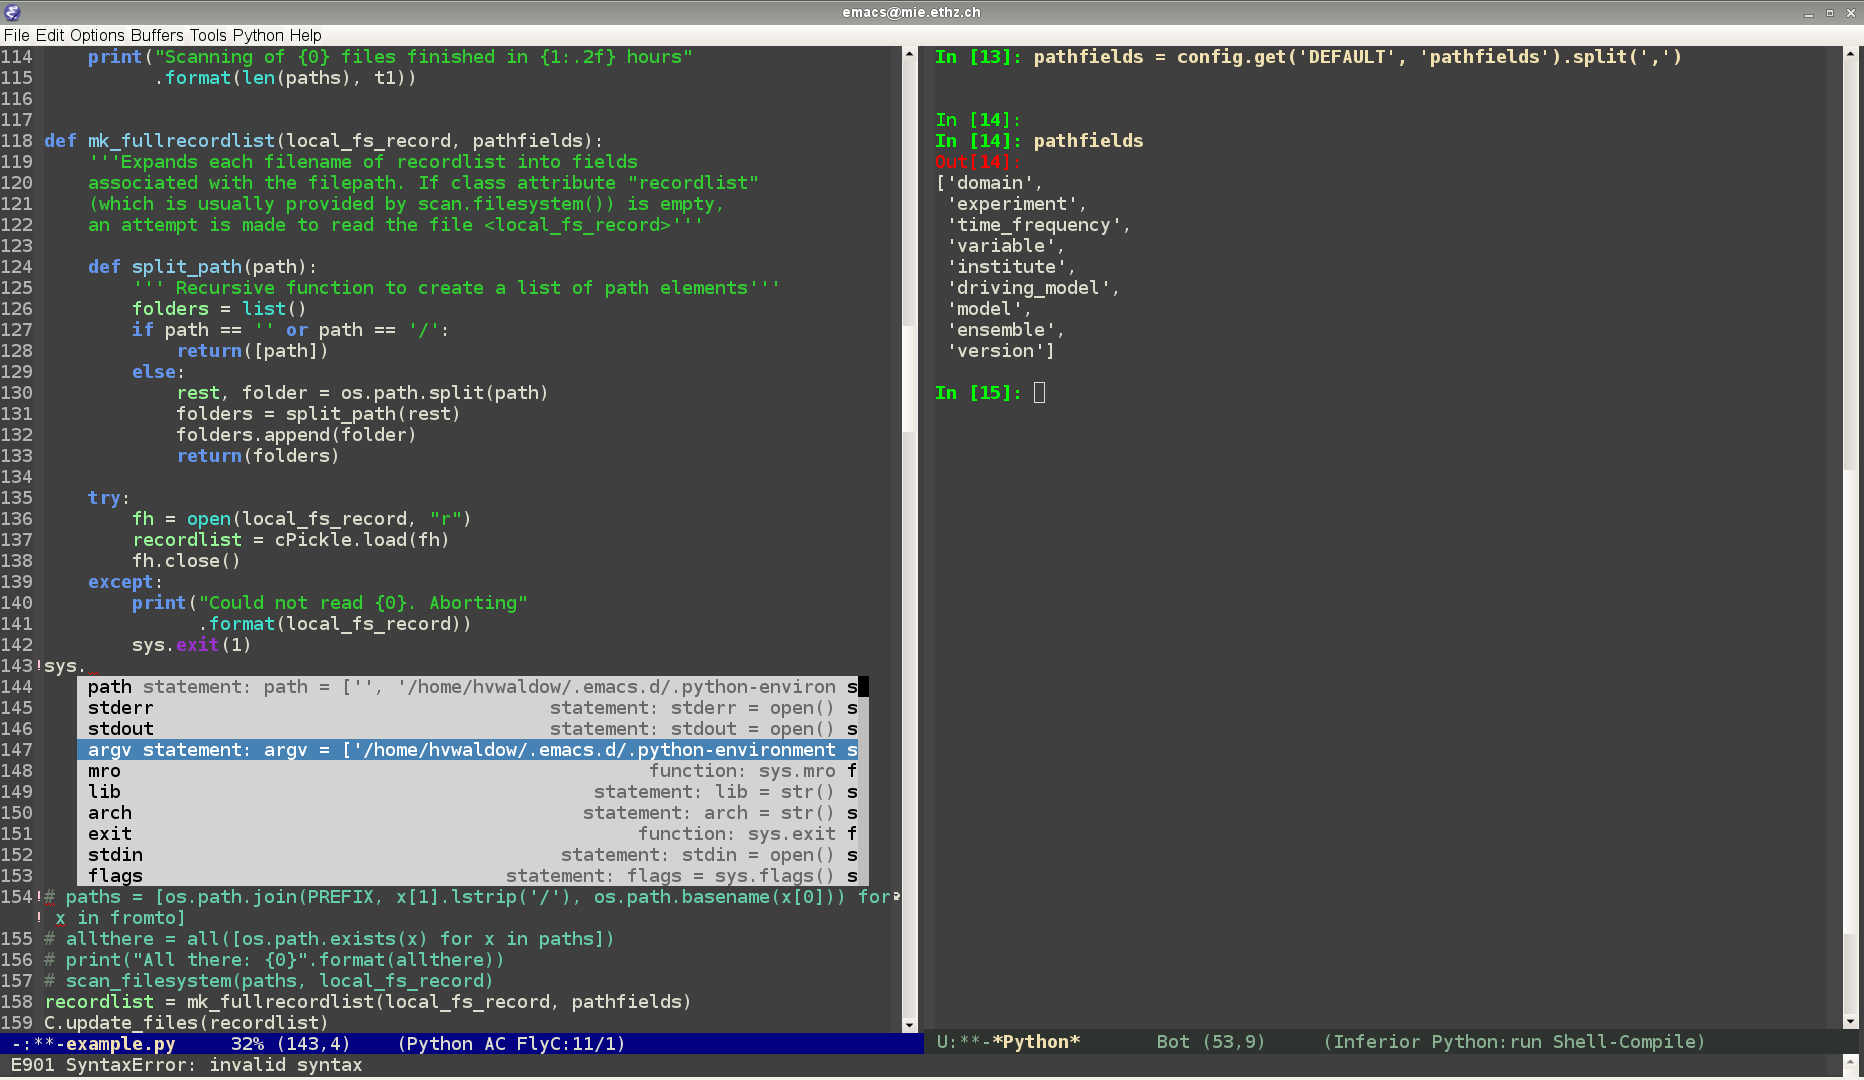
\includegraphics[width=\textwidth]{emacs.png}
  \end{block}
\end{frame}

\begin{frame}
  \frametitle{Python development tools}
  \begin{block}{Editors with plugins}
    \begin{itemize}
    \item<1-> Emacs
    \item<1-> Vim
    \item<1-> other editors with varying degrees of support
    \item<1-> Geany, TextWrangler, \ldots
    \item<2-> More screen-estate for code \& interpreter
    \item<2-> Keyboad instead of mouse $\Rightarrow$ faster!
    \item<2-> Might be complicated to set up, initially.
    \item<2-> Steeper learning curve
    \item<3-> \alert{If you already use Emacs or Vim, go for it!}
    \end{itemize}
  \end{block}
\end{frame}


\begin{frame}
  \frametitle{Python development tools}
  \begin{block}{And now for something completely different \ldots}
    \begin{overprint}
    \onslide<1>{\centering 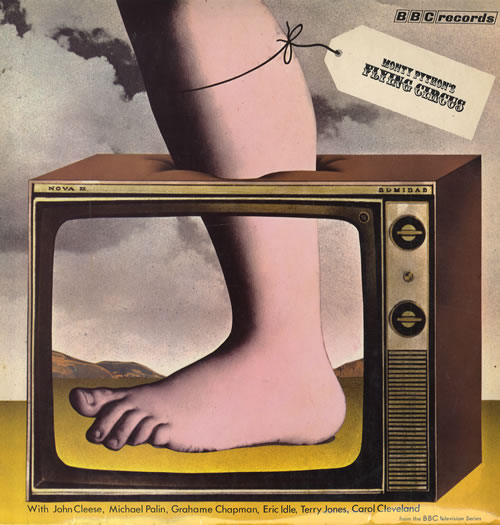
\includegraphics[height=0.75\textheight]{monty.jpg}\\}
    \end{overprint}
  \end{block}
\end{frame}

\usebackgroundtemplate{}

\begin{frame}
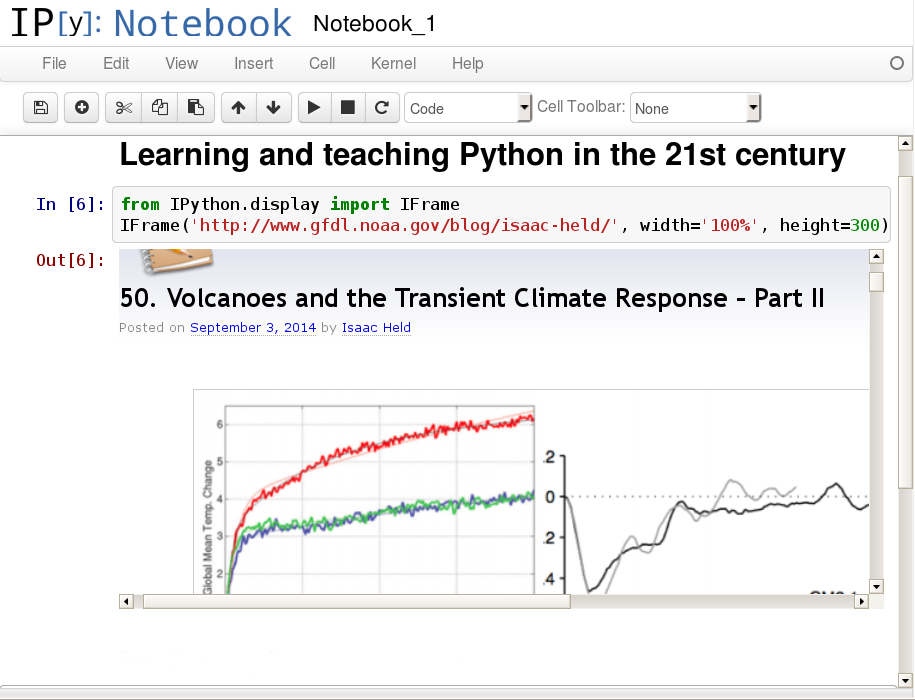
\includegraphics[height=\textheight]{notebook.png}
\end{frame}

\end{document}
